\documentclass[10pt]{article}
\usepackage{fullpage}
\usepackage{amsmath}
\usepackage[amsthm, thmmarks]{ntheorem}
\usepackage{amssymb}
\usepackage{graphicx}
\usepackage{epstopdf}

\newtheorem{lemma}{Lemma}[section]
\newtheorem{theorem}[lemma]{Theorem}
\newtheorem{definition}[lemma]{Definition}
\newtheorem{proposition}[lemma]{Proposition}
\newtheorem{claim}[lemma]{Claim}
\newtheorem{corollary}[lemma]{Corollary}

\newcommand{\dee}{\mathrm{d}}
\newcommand{\In}{\mathrm{in}}
\newcommand{\Out}{\mathrm{out}}
\newcommand{\pdf}{\mathrm{pdf}}
\newcommand{\Ei}{\mathrm{Ei}}

\title{Random Walk and Electrical Networks}
\author{Pramook Khungurn}

\begin{document}
	\maketitle
	
\section{Random Walks in One Dimension}

\begin{itemize}
	\item Consider a random walk on integers $0, 1, 2, \dotsc, N$.
		
		Let $p(x)$ be the probability that, starting at $x$,
		the walker reach $N$ before reading $0$.
		
		We have that:
		\begin{itemize}
			\item $p(0) = 0.$
			\item $p(N) = 1.$
			\item $p(x) = \frac{1}{2} p(x-1) + \frac{1}{2} p(x+1)$
				for all $x$ such that $1 \leq x \leq N-1.$
		\end{itemize}
		
	\item Consider an electrical network in Figure~\ref{1d-network}.
	
	\begin{figure}[h]
		\centering
		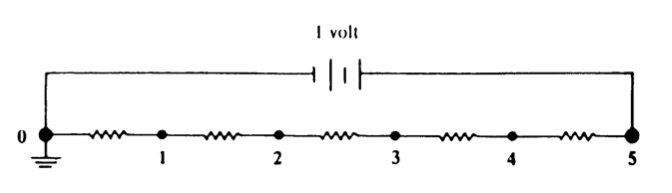
\includegraphics[width=4in]{1d-network.png}
		\caption{A 1D electrical network. Each resistor is 1 Ohm.}
		\label{1d-network}		
	\end{figure}
	
	Let $v(i)$ denote the voltage at point $i$. We have that
	\begin{itemize}
		\item $v(0) = 0$.
		\item $v(5) = 1$.
	\end{itemize}
	
	\item We will derive expressions for voltage at other points
		by laws of electrical networks. So, it is good to review
		those laws now. We will be using two laws:
		
		\begin{itemize}
			\item {\bf Ohm's Law.} The current flowing through
			a resister $R$ connecting points $x$ and $y$ in
			the direction from $x$ to $y$ is
			by $$\frac{v(x) - v(y)}{R}.$$
			
			\item {\bf Kirchhoff's Current Law.} The current flowing
			out of any point in an electrical circuit is always zero.
		\end{itemize}
	
	\item Let us go back to the electrical network in Figure~\ref{1d-network}.
		We have that the current flowing out of $x$ is given by
		$$\frac{v(x) - v(x+1)}{1} + \frac{v(x) - v(x-1)}{1} 
		= 2v(x) - v(x+1) - v(x-1).$$
		By Kirchhoff's Current Law, the above expression is $0$.
		In other words,
		$$v(x) = \frac{1}{2} v(x-1) + \frac{1}{2} v(x+1)$$
		for any $x = 1, 2, \dotsc, N-1.$
	
	\item We can see that $p$ and $v$ are very similar. In turns out
		that we can show that they must be the same.
\end{itemize}

\section{Harmonic Functions in One Dimension}

\begin{itemize}
	\item Let $S = \{0, 1, 2, \dotsc, N\}$. 
		
		We call the points in the set $D = \{1, 2, \dotsc, N-1\}$ 
		the \emph{interior points}, and the points in 
		$B = \{0, N\}$ the \emph{boundary points}.
		
	\item \begin{definition}
		A function $f$ defined on $S$ is \emph{harmonic} if
		$$f(x) = \frac{f(x-1) + f(x+1)}{2}$$ for all $x \in D$.
		In other words, $f(x)$ is the average of its neighbors.
	\end{definition}
	
	\item We can see from the last section that $p$ and $v$
		are harmonic functions. We also see that they have
		the same boundary values. That is, $p(0) = v(0) = 0$
		and $p(N) = v(N) = 1.$
		
	\item We shall determine whether $p$ and $v$ are actually
		the same. The tool that lets us do that is the following
		\emph{maximum principle}.
		
		\begin{lemma}[Maximum Principle]
			A harmonic function $f(x)$ defined on $S$ takes
			on its maximum value $M$ and its minimum value $m$
			on the boundary.
		\end{lemma}
		
		\begin{proof}
			Suppose by way of contradiction that $f$
			takes on its maximum value $M$ at an interior point
			$x$. Moreover, assume that $f(x) > f(0)$ and 
			$f(x) > f(N).$ Then, because $f(x)$ is the average
			of $f(x-1)$ and $f(x+1)$, one of $f(x-1)$ and
			$f(x+1)$ must be at least $M$. Continuing this way,
			we have that $f(0)$ or $f(N)$ must be equal to $M$,
			a contradiction.
			
			The same argument also works for $m$.
		\end{proof}
		
	\item \begin{corollary} \label{constant-harmonic-function}
		If $f$ is a harmonic function such that $f(0) = c$
		and $f(N) = c$ for some constant $c$, then $f(x) = c$
		for all $x \in S.$
	\end{corollary}
	
	\item Finding harmonic functions that having specified boundary
		values is called the \emph{Dirichlet problem.} The 
		\emph{uniqueness principle} states that there can be
		only one solution to the \emph{Dirichlet problem}.
		
		\begin{theorem}[Uniqueness Principle]
			If $f$ and $g$ are harmonic functions such that
			$f(0) = g(0)$ and $f(N) = g(N),$ then $f = g$.
		\end{theorem}
		
		\begin{proof}
			Let $h = f - g.$ We have that $h$ is a harmonic
			function, and $h(0) = h(N) = 0.$
			By Corollary~\ref{constant-harmonic-function},
			$h(x) = 0$ for all $x$, which means that
			$f(x) = g(x)$ for all $x$.
		\end{proof}
	
	\item Returning to the random walk and the electrical network
		in the last section, we have that $p = v$.
\end{itemize}

\end{document}